%; whizzy paragraph -pdf xpdf -latex ./whizzypdfptex.sh
%; whizzy-paragraph "^\\\\begin{frame}\\|\\\\emtext"
% latex beamer presentation.
% platex, latex-beamer でコンパイルすることを想定。 

%     Tokyo Debian Meeting resources
%     Copyright (C) 2012 Junichi Uekawa
%     Copyright (C) 2012 Nobuhiro Iwamatsu

%     This program is free software; you can redistribute it and/or modify
%     it under the terms of the GNU General Public License as published by
%     the Free Software Foundation; either version 2 of the License, or
%     (at your option) any later version.

%     This program is distributed in the hope that it will be useful,
%     but WITHOUT ANY WARRANTY; without even the implied warreanty of
%     MERCHANTABILITY or FITNESS FOR A PARTICULAR PURPOSE.  See the
%     GNU General Public License for more details.

%     You should have received a copy of the GNU General Public License
%     along with this program; if not, write to the Free Software
%     Foundation, Inc., 51 Franklin St, Fifth Floor, Boston, MA  02110-1301 USA

\documentclass[cjk,dvipdfmx,12pt]{beamer}
\usetheme{Tokyo}
\usepackage{monthlypresentation}

\setbeamertemplate{footline}{\hskip1mm\insertshortdate\hfill\hbox{\insertpagenumber /\insertdocumentendpage }\hspace*{1mm}\vskip1mm}

\newcommand<>{\fullsizegraphic}[1]{
  \begin{textblock*}{0cm}(-1cm,-3.78cm)
  \includegraphics[width=\paperwidth]{#1}
  \end{textblock*}
}

\newcommand<>{\minisectiontilte}[2]{
  {\fontsize{40pt}{40pt}\selectfont\color{#1}#2}
}


%  preview (shell-command (concat "evince " (replace-regexp-in-string "tex$" "pdf"(buffer-file-name)) "&")) 
%  presentation (shell-command (concat "xpdf -fullscreen " (replace-regexp-in-string "tex$" "pdf"(buffer-file-name)) "&"))
%  presentation (shell-command (concat "evince " (replace-regexp-in-string "tex$" "pdf"(buffer-file-name)) "&"))

%http://www.naney.org/diki/dk/hyperref.html
%日本語EUC系環境の時
\AtBeginDvi{\special{pdf:tounicode EUC-UCS2}}
%シフトJIS系環境の時
%\AtBeginDvi{\special{pdf:tounicode 90ms-RKSJ-UCS2}}

\title{東京エリアDebian勉強会}
\subtitle{第91回 2012年9月度/OSC2012 Tokyo/Fall)}
\author{岩松 信洋\\iwamatsu@debian.org}
\date{2012年9月8日}
\logo{
\includegraphics[width=8cm]{image200607/openlogo-light.eps}}

\begin{document}

\frame{\titlepage{}}

\begin{frame}{自己紹介}

\begin{itemize}
\item 岩松 信洋 / Nobuhiro Iwamatsu
\item Twitter / @iwamatsu
\item Debian Project Official Developer
\item Linux kernel, Debian/SuperH, Bluetooth subsystem, Debian Science (OpenCV), Mozc, etc...
\item 普段は Linux kernel 開発、ブートローダ開発、などをしています
\end{itemize}

\end{frame}

\begin{frame}[plain]

\begin{center}
Git の本とか書きました。買ってね。
%\includegraphics[width=0.5\hsize]{image201209/gitbook.jpg}
\end{center}

\end{frame}
% gitbook.jpg
% http://ecx.images-amazon.com/images/I/51WQ7GsnOZL._SL300_.jpg


\begin{frame}{注意事項}
\begin{itemize}
  \item 疑問、質問、ツッコミ 大歓迎
  \item その場でインタラクティブにどうぞ
\end{itemize}
\end{frame}

\emtext{今回のお話}

{
% 画面全体に画像を張りた場合には、\frame{}の前に\setbeamertemplate{background canvas} 
% を使って画像を指定し、frame には plain を指定する。

%\setbeamertemplate{background canvas}{} 

%\setbeamertemplate{background canvas}{\includegraphics[width=\paperwidth]{image201209/1000px-Wheezy3.jpg}} 
\begin{frame}[plain]%{今日のお話}

\begin{center}
\pause
{\fontsize{40pt}{40pt}\selectfont\color{red}Wheezy}
%\Huge{\color{red}{次期安定版 Debian 7.0 "Wheezy" について}}

\end{center}

\end{frame}
}

\begin{frame}[containsverbatim]{Debian 7.0 "Wheezy" is now under freeze}

\begin{commandline}

To: debian-devel-announce@lists.debian.org
Subject: 5... 4... 3... 2... 1...
From: "Adam D. Barratt" <adam@adam-barratt.org.uk>
Date: Sat, 30 Jun 2012 21:20:55 +0100

Hi, 

As previously announced[1], testing is now frozen.

- snip -
Adam,
for the Debian Release Team

\end{commandline}

\end{frame}

\begin{frame}{アジェンダ}
\begin{itemize}
 \item  「で、Wheezyってどうよ?」\\
   Debian 7.0 "Wheezy" の変更点、現状
 \item 「ところで次のリリースは?」\\
   次期リリース Debian 8.0(?) へ向けて
\end{itemize}
\end{frame}

\begin{frame}{アジェンダ}
\begin{itemize}
 \item {\color{red}「フリーズって何?」 \\
  Debian のリリースサイクルについて}
 \item  「で、Wheezyってどうよ?」\\
   Debian 7.0 "Wheezy" の変更点、現状
 \item 「ところで次のリリースは?」\\
   次期リリース Debian 8.0(?) へ向けて
\end{itemize}
\end{frame}

\section{フリーズって何?}

\emtext{フリーズって何?}

\begin{frame}
\begin{center}
\minisectiontilte{black}{Debian Infographics}
\end{center}
\end{frame}

{
%\setbeamertemplate{background canvas}{} 
\setbeamertemplate{background canvas}{\includegraphics[width=\paperwidth]{image201209/infographic_debian-ja-v1-1.png}}
\begin{frame}[plain]%{Debian Infographics}
\end{frame}
}

\begin{frame}{Debianの「ディストリビューション」}

\begin{itemize}
\item 3つの「ディストリビューション」\\
  stable, testing, unstable
\item ディストリビューション以外の「リポジトリ」\\
  updates(旧volatile), security-updates \\
  backports, experimental \\
\end{itemize}

\end{frame}

\begin{frame}
\begin{center}
\minisectiontilte{black}{Debianのリリースサイクル}
\end{center}
\end{frame}

{
\setbeamertemplate{background canvas}{\includegraphics[width=\paperwidth]{image201011/Debian-Release-Cycle01.png}}
\begin{frame}[plain]%{Debianのリリースサイクル / 1}
\end{frame}
}

{
\setbeamertemplate{background canvas}{\includegraphics[width=\paperwidth]{image201011/Debian-Release-Cycle02.png}}
\begin{frame}[plain]%{Debianのリリースサイクル / 2}
\end{frame}
}

{
\setbeamertemplate{background canvas}{\includegraphics[width=\paperwidth]{image201011/Debian-Release-Cycle03.png}}
\begin{frame}[plain]%{Debianのリリースサイクル / 3}
\end{frame}
}

{
\setbeamertemplate{background canvas}{\includegraphics[width=\paperwidth]{image201011/Debian-Release-Cycle04.png}}
\begin{frame}[plain]%{Debianのリリースサイクル / 4}
\end{frame}
}

{
\setbeamertemplate{background canvas}{\includegraphics[width=\paperwidth]{image201011/Debian-Release-Cycle05.png}}
\begin{frame}[plain]%{Debianのリリースサイクル / 5}
\end{frame}
}

\begin{frame}

\begin{center}
\minisectiontilte{black}{よくある誤解}
\end{center}

\end{frame}

\begin{frame}{今までのリリースサイクル}

\begin{center}
%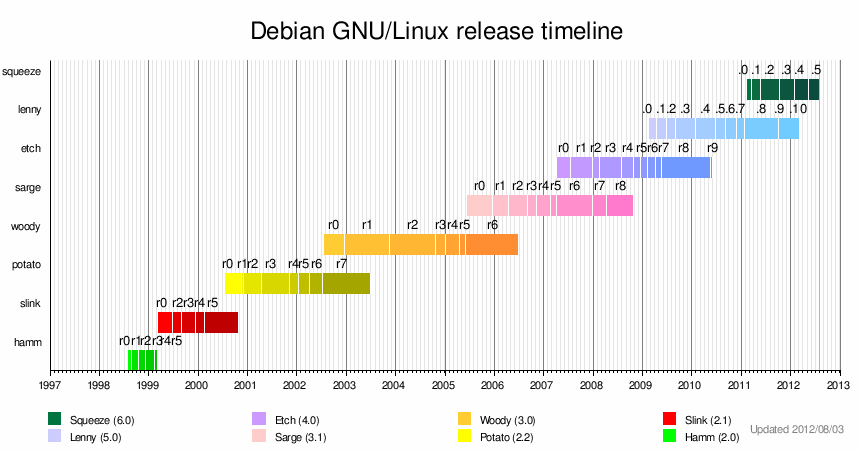
\includegraphics[width=1\hsize]{image201209/e0247344d383734858d7d2099e9037bc.png}
\end{center}

\end{frame}

\begin{frame}{今までのリリースサイクル}

\begin{itemize}
\item Debianのリリースは予測不可能/遅れるのが当たり前
\item \color{red}{Etch から ほぼ 2 年毎のリリース}
\begin{itemize}
  \item 3.1 "Sarge"   : 約 3 年
  \item 4.0 "Etch"    : 22ヶ月
  \item 5.0 "Lenny"   : 22ヶ月
  \item 6.0 "Squeeze" : 24ヶ月
\end{itemize}
\end{itemize}

\end{frame}

\begin{frame}{今までのリリースサイクル}

\begin{itemize}
\item \sout{Debianのリリースは予測不可能/遅れるのが当たり前}
\item \color{red}{Etch から ほぼ 2 年毎のリリース}
\begin{itemize}
  \item 3.1 "Sarge"   : 約 3 年
  \item 4.0 "Etch"    : 22ヶ月
  \item 5.0 "Lenny"   : 22ヶ月
  \item 6.0 "Squeeze" : 24ヶ月
\end{itemize}
\end{itemize}

\end{frame}

\begin{frame}{Time Based Release Freeze}

\begin{center}
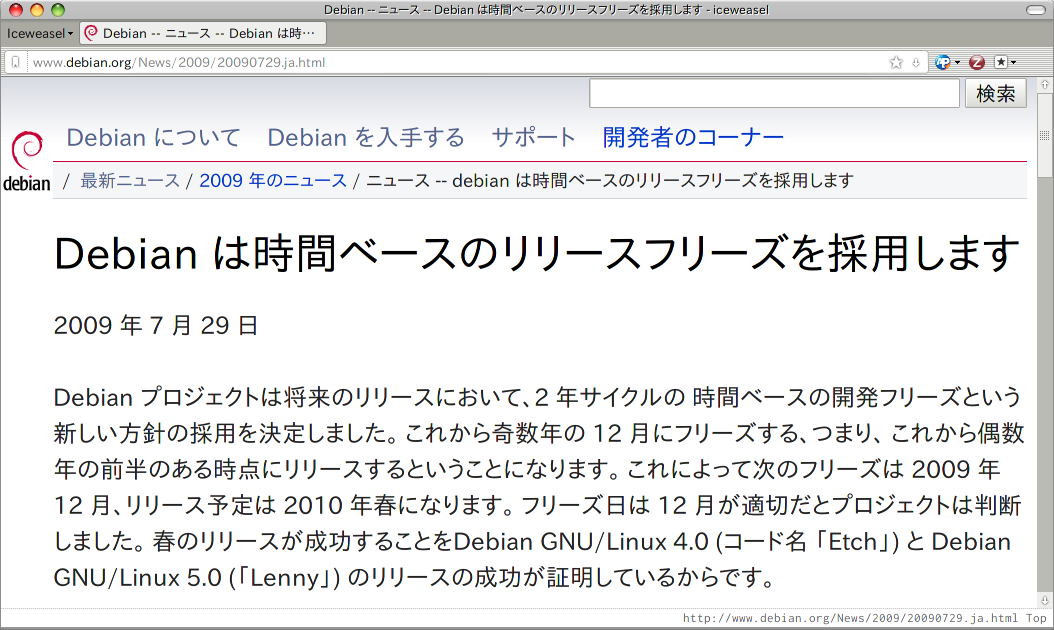
\includegraphics[width=1\hsize]{image201208/Debian_News_2009-07-29-TimeBasedReleaseFreeze.png}
\end{center}

\end{frame}

\begin{frame}{Time Based Release Freeze}

\begin{itemize}
\item testing の フリーズは2年単位になった!!
  \begin{itemize}
    \item Squeeze の Freeze / 2010/08/06 \\$\rightarrow$ 2011/02/06 リリース!
    \item Wheezy の Freeze 2012/06/30 \\$\rightarrow$ 2012/12?
  \end{itemize}
\item 利点:
  \begin{itemize}
    \item 使用者: リリースの時期を予測できる
    \item 開発者: 長期プランを立てやすくなる
  \end{itemize}
\end{itemize}

\end{frame}

\begin{frame}{まとめ: Debian のリリースサイクル}

\begin{itemize}
  \item Debian = 常に進化し続けるディストリビューション
  \begin{itemize}
    \item stable, testing, unstable
    \item 頑健な「stable」と最前線を疾走する「unstable」
  \end{itemize}
  \item Time Based Release Freeze
  \begin{itemize}
    \item \sout{「リリースが遅い/読めない」}→約二年毎の安定版のリリース
    \item 定期的なリリースフリーズによる "huge jump" の回避
  \end{itemize}
\end{itemize}

\end{frame}


\begin{frame}

\begin{center}
\minisectiontilte{black}{何か質問はありますか?}
\end{center}

\end{frame}

\section{Debian "7.0" Wheezy}
\emtext{Debian "7.0" Wheezy}

{
% 画面全体に画像を張りた場合には、\frame{}の前に\setbeamertemplate{background canvas} 
% を使って画像を指定し、frame には plain を指定する。

%\setbeamertemplate{background canvas}{} 
%\setbeamertemplate{background canvas}{\includegraphics[width=\paperwidth]{image201209/1000px-Wheezy3.jpg}} 
\begin{frame}[plain]%{今日のお話}
\end{frame}
}

{
%\setbeamertemplate{background canvas}{\includegraphics[width=\paperwidth]{image201209/stop_time_by_curlydeea-d4poj4p.jpg}} 
\begin{frame}[plain]

\huge{
\begin{itemize}
  \item \color{red}{2012/06/30 にフリーズ!! $\rightarrow$ 現在は}{\color{green}frozen}
  \item \color{red}{リリースに向けたバグ(RCバグ)潰しが進行中}
\end{itemize}
}
\end{frame}
}
%%http://www.ethansenglishcafe.com/wp-content/uploads/2012/04/stop_time_by_curlydeea-d4poj4p.jpg

{
\setbeamertemplate{background}{\includegraphics[width=\paperwidth]{image201011/Debian-Release-Cycle04.png}}
\begin{frame}[plain]
\begin{center}
\pause
{\fontsize{40pt}{40pt}\selectfont\color{red}{いまここ!}}
\end{center} 
\end{frame}
}


\begin{frame}

\begin{center}
\minisectiontilte{black}{RC バグ数}
\end{center}

\end{frame}

{
\setbeamertemplate{background canvas}{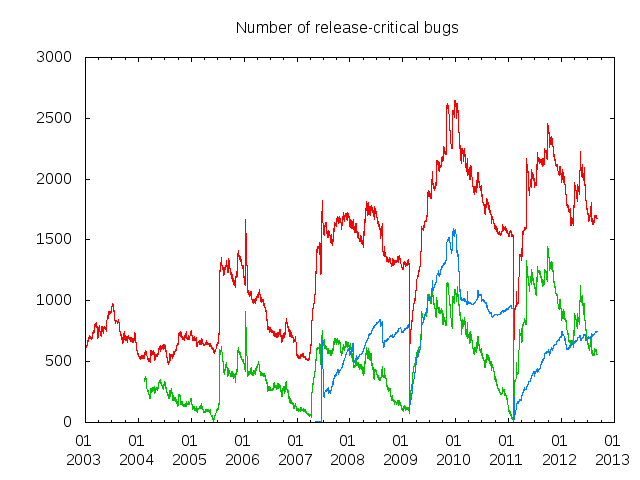
\includegraphics[width=\paperwidth]{image201209/graph.png}}
\begin{frame}[plain]%{RC バグ数}

\begin{center}
\pause
{\fontsize{40pt}{40pt}\selectfont 2012/09/08 現在 \\RC バグ: 540}
\end{center}

\end{frame}
}


\begin{frame}{RC バグ}

\begin{itemize}
  \item 540バグのうち\pause
  \item パッチがあるバグ: 108
  \item 無視されるバグ: 29
  \item あと300個ぐらい\pause
  \item みなさん、がんばりましょう
  
\end{itemize}


\end{frame}



\begin{frame}

\begin{center}
\minisectiontilte{black}{Wheezy のリリースゴール}
\end{center}

\end{frame}


\begin{frame}{Wheezy のリリースゴール}

\begin{itemize}
  \item Multiarch への移行
  \item kFreeBSD (← テクノロジープレビューだった)
  \item IPv6 完全サポート
  \item ラージファイルサポート
  \item .la ファイルの削除
\end{itemize}

\end{frame}



\begin{frame}{Wheezy のリリースゴール}

\begin{itemize}
  \item {\color{red}Multiarch への移行}
  \item kFreeBSD (← テクノロジープレビューだった)
  \item IPv6 完全サポート
  \item ラージファイルサポート
  \item .la ファイルの削除
\end{itemize}

\end{frame}



\begin{frame}{Multiarch}

\begin{itemize}
  \item 同一のシステム上で、異なるハードウェアアーキテクチャのライブラリ等をインストールする仕組み\\
  /usr/lib/ $\rightarrow$ /usr/lib/x86\_64-linux-gnu\\
  \item 何が嬉しいのか?
  \begin{itemize}
    \item 類似のアーキテクチャを一緒に動作させることができる\\
    $\rightarrow$ i386 on amd64, armel on armhf \\
    \item クロスビルド環境の構築が容易になる
  \end{itemize}
\end{itemize}

\end{frame}

\begin{frame}[containsverbatim]{Multiarch: どうやって?}

\begin{commandline}
# dpkg --add-architecture i386
# dpkg --print-foreign-architectures
i386
# echo "deb [arch=i386,amd64] \
  http://ftp.jp.debian.org/debian/ wheezy main" \
   > /etc/apt/sources.list
# apt-get update
# apt-get install libc6:i386   
# dpkg --remove-architecture i386
\end{commandline}
%$
%\footnote{\url{http://wiki.debian.org/ReleaseGoals/MultiArch}}

\end{frame}


\begin{frame}{Wheezy のリリースゴール}

New for Wheezy
\begin{itemize}

  \item Security hardening build flags
  \item /run への移行
  \item Video4Linux1 を使っているパッケージの修正および削除
  \item /dev/dsp を使っているパッケージの修正および削除
\end{itemize}

\end{frame}


\begin{frame}{Wheezy のリリースゴール}

New for Wheezy
\begin{itemize}

  \item {\color{red}{Security hardening build flags}}
  \item /run への移行
  \item Video4Linux1 を使っているパッケージの修正および削除
  \item /dev/dsp を使っているパッケージの修正および削除

\end{itemize}

\end{frame}


\begin{frame}{Security hardening build flags}
パッケージ構築時にセキュリティを強化するコンパイルフラグを(デフォルトで)有効にする。

\begin{itemize}
  \item Format string checks( -Wformat -Werror=format-security )\\
  format 使う関数(例えば printf)の使用が問題を引き起こす可能性がある場合に警告する。
  \item FORTIFY\_SOURCE \\
  文字列やメモリの操作を行う関数を使用する際にバッファオーバーフローを検出する。

\end{itemize}

\end{frame}



\begin{frame}{Security hardening build flags}
パッケージ構築時にセキュリティを強化するコンパイルフラグを(デフォルトで)有効にする。

\begin{itemize}
  \item -fstack-protector --param=ssp-buffer-size=4 \\
  スタック破壊攻撃等によるバッファオーバーフローをチェックするための追加コードを生成する。
  4バイトを超える配列を持つ関数を対象にする。
  \item -z,now,-z,relro \\
  リロケーション領域(GOTなど)をリードオンリーにする。
\end{itemize}

\end{frame}


\begin{frame}{Wheezy のリリースゴール}

New for Wheezy
\begin{itemize}

  \item Security hardening build flags
  \item {\color{red}{/run} への移行}
  \item Video4Linux1 を使っているパッケージの修正および削除
  \item /dev/dsp を使っているパッケージの修正および削除

\end{itemize}

\end{frame}


\begin{frame}{/run}

boot の早い段階で一時ディレクトリを用意
\begin{itemize}
  \item /var/run → /run
  \item /var/lock → /run/lock
  \item /dev/shm → /run/shm
  \item /tmp → /run/mp
\end{itemize}

\end{frame}

\begin{frame}
\begin{center}
\minisectiontilte{black}{主なパッケージのバージョン}
\end{center}
\end{frame}

\begin{frame}{主なパッケージのバージョン / 1}

\begin{itemize}
  \item Kernel: Linux 3.2, Freebsd 8.3, 9.0
  \item libc: eglibc 2.13
  \item GNU Compiler Collection: 4.7.1 (i386/amd64のみ)、4.6.3 (i386/amd64 以外)
  \item OpenJDK: 6b24-1.11.3, 7$~$u3-2.1.1
\end{itemize}

\end{frame}

\begin{frame}{主なパッケージのバージョン / 2}

\begin{itemize}
  \item  Xorg X11R7.7
  \item  GNOME 3.4, KDE 4.8, Xfce 4.8
  \item  Iceweasel 10.0.6esr-1, icedove 10.0.5-1
  \item  LibreOffice 3.5.4
  \item  GIMP 2.8.0, Inkscape 0.48.3.1
\end{itemize}

\end{frame}

\begin{frame}{主なパッケージのバージョン / 3}

\begin{itemize}
  \item Apache httpd 2.2.22, Samba 3.6.6, 4.0.0~beta2
  \item PostgreSQL 8.4.12, MySQL 5.5.24
  \item Xen Hypervisor 4.1.3~rc1
  \item Python 2.7, 2.6, and 3.2, Perl 5.14.2
  \item Ruby 1.9.3p194, 1.8.7.358 \\
        1.8 will be dropped in Wheezy+1
\end{itemize}

\end{frame}

\begin{frame}{その他の変更点}

\begin{itemize}
 \item Linux RT kernel サポート
 \item Xen Cloud Platform (XCP)、Openstack サポート 
 \item New ports\\
  armhf, s390x
 \item Debian Installer の改善 \\
  WPA サポート(ファームウェアは別配布)
 \item  New Artwork: "Joy"
\end{itemize}

\end{frame}

\begin{frame}{その他の変更点}

\begin{itemize}
 \item Linux RT kernel サポート
 \item Xen Cloud Platform (XCP)、Openstack サポート 
 \item New ports\\
  armhf, s390x
 \item Debian Installer の改善 \\
  WPA サポート(ファームウェアは別配布)
 \item  {\color{red}New Artwork: "Joy"}
\end{itemize}

\end{frame}


{
\begin{frame}[plain]

\begin{center}
\minisectiontilte{black}{Joy?}
\end{center}

\end{frame}
}

\begin{frame}[plain]
\begin{center}
%\includegraphics[width=1\hsize]{image201209/joy.jpg}
\end{center}
\end{frame}


{
\setbeamertemplate{background canvas}{
\includegraphics[width=\paperwidth]{image201209/debian-joy-xga.png}}
\begin{frame}[plain]
\begin{center}
\end{center}

\end{frame}
}


\begin{frame}{まとめ: Debian 7.0 "Wheezy" の状況}

\begin{itemize}
  \item Wheezy \\
  frozen → 現在はリリースに向けたバグ修正中
  \item ユーザ向けの大きな変更点\\
  \begin{itemize}
    \item Multiarch, /run, ... 
    \item アートワーク, インストーラの改善... 
  \end{itemize}
\end{itemize}

\end{frame}

\begin{frame}

\begin{center}
\minisectiontilte{black}{何か質問はありますか?}
\end{center}

\end{frame}

\section{ところで次は?}
\emtext{ところで次は?}


{
\begin{frame}[plain]

\begin{center}
\pause
\minisectiontilte{red}{コードネーム: Jessie}
\end{center}

\end{frame}
}


\begin{frame}[plain]
\begin{center}
%\includegraphics[width=1\hsize]{image201209/mae.png}
\end{center}
\end{frame}


{
%\setbeamertemplate{background canvas}{\includegraphics[width=\paperwidth]{image201209/Jessiewallpaper1.jpg}}
\begin{frame}[plain]

\begin{center}
\pause
\minisectiontilte{red}{Jessie}
\end{center}

\end{frame}
}


\begin{frame}[plain]
\begin{center}
%\includegraphics[width=1\hsize]{image201209/ato.png}
\end{center}
\end{frame}

\begin{frame}

\begin{center}
\Huge{初の女キャラクター!}\\\pause
\Huge{他は特になし}
\end{center}
\end{frame}


\emtext{Wheezyのリリースに向けて}

\begin{frame}[plain]
\begin{center}
%
\includegraphics[width=0.8\hsize]{image201209/I_want_you.jpg}
\end{center}
\end{frame}

\begin{frame}{Wheezyのリリースに向けて}

\begin{itemize}
  \item Wheezy を{\color{red}{是非}}試してみて下さい!!
  \begin{itemize}
    \item Squeeze からのアップグレード/使ってみてレポートなど.
    \item  Debian BTS: http://www.debian.org/Bugs/
  \end{itemize}
  \item ドキュメントの翻訳者も募集してます!!:
  \item ニュース/リリースノート...
\end{itemize}

\end{frame}

\begin{frame}[plain]

\begin{center}
\minisectiontilte{red}{どうしていいかわからない!}
\end{center}

\end{frame}


\begin{frame}{そんな貴方に}

\begin{itemize}
  \item Debian 勉強会
  \begin{itemize}
    \item Debianのユーザと開発者がface to faceで話し合う場
    \item Debian開発者および開発者予備軍を育成する場
    \item Debianの最新情報、バッドノウハウを提供する場
    \item 東京エリア(関東) と関西で月に1回開催中
    \item \url{http://tokyodebian.alioth.debian.org}
  \end{itemize}
\end{itemize}

\end{frame}

\begin{frame}{東京エリアDebian勉強会}

\begin{itemize}
  \item 毎月第三土曜日。 18:00-21:00 ぐらい
  \item 荻窪、新宿 など
  \item 次回は10月20日、朝日ネットさん
  \item 関西、福岡方面でも勉強会やっています。
\end{itemize}

\end{frame}

\begin{frame}{Debian パッケージング道場}

\begin{itemize}
  \item Debian パッケージングを伝授する道場
  \item Debianへのインストールまでサポート(すごい!)
  \item 第0回は 9月22日 楽天さんで開催
  \item http://www.zusaar.com/event/355109
\end{itemize}

\end{frame}


\begin{frame}{Debian Hack Cafe}

\begin{itemize}
  \item 結婚や就職と引換にDebian開発時間をなくした開発者が集まってわいわいといろいろ開発する集まり
  \item 場所は新宿近辺。
  \item 詳細な場所時間は Twitter  / @debian\_hackcafe で通知。
\end{itemize}

\end{frame}

\begin{frame}{Debian パッケージをいじる会}

\begin{itemize}
  \item Debian パッケージをいじる会
  \item 五反田近辺で開催。
\end{itemize}

\end{frame}

\begin{frame}

\begin{center}
\minisectiontilte{black}{何か質問はありますか?}
\end{center}

\end{frame}

\begin{frame}{Debianブースのお知らせ}

\begin{itemize}

  \item 展示
  \begin{itemize}
    \item Wheezyの実機を展示しています。
    \item Debian Infographics(日本語版)配布しています。
  \end{itemize}

  \item 販売、配布
  \begin{itemize}
    \item 日本唯一の Debian 専門同人誌 あんどきゅめんてっどでびあん
    \item Debian ステッカー
    \item Debian 7.0 (bata 1) インストールCD  
  \end{itemize}

\end{itemize}

\end{frame}

\begin{frame}

\begin{center}
\minisectiontilte{black}{ありがとうございました。}
\end{center}

\end{frame}



\end{document}

;;; Local Variables: ***
;;; outline-regexp: "\\([ 	]*\\\\\\(documentstyle\\|documentclass\\|emtext\\|section\\|begin{frame}\\)\\*?[ 	]*[[{]\\|[]+\\)" ***
;;; End: ***
